\chapter{Introduction to Event Streaming}

In previous chapter we defined what a message broker basically is, therefore we
can imagine how Apache Kafka works. Because Apache Kafka is build for big data
environments \todo{big data erklären} concepts like events and streams become
important. To understand the possible use cases of Apache Kafka, the terms
around event streaming need to be clarified. 

\begin{figure}[H]
    \centering
    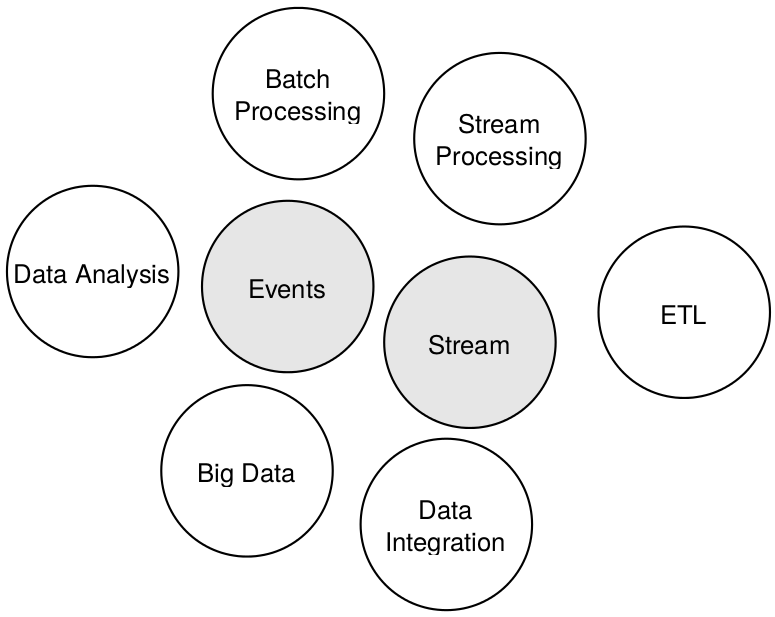
\includegraphics[width=0.45\textwidth]{images/evenstreaming-intro.png}
    \caption{Event Streaming terms}
    \label{fig:evenstreaming-intro}
\end{figure}

\section{Purpose}
The view of data as rows of databases or single files changes when one thinks
about what a business actually does with the generated data. Where retail
generates orders they lead to sales, shipments and so on, a financial
institution will generate orders they are going to have an impact of a stock
price. Or a social network platform generates clicks, impressions and searches
they are used to make some sort of intelligent analysis to further display
personalized data to it's users. Such kind of data can be thought of as streams
of events. In fact, collecting all events a business ever generated will lead to
the current state of the business and thus describe what the business did in
past. For example the current price of a stock was generated by all the orders
ever made on this stock. Every order can be captured as an event and so can all
events together reproduce the current stock price.

\section{What is an Event?}
\label{intro-datastream-datastream}
Very basically an event occurs when "something happens"  in a system like when a
user of an online shop adds an item to its basket. In modern systems, events are
transmitted as discrete messages on a MOM (see \ref{intro-messaging-mom}) and
thus following Tannenbaum et al. (2006), represent a data unit of a data
streams. Where a data stream can be applied to discrete as well as continuous
media, events are transmitted as discrete messages only. The message itself
can be considered as an event message \cite{EIP03}.

If we think more traditionally, even database systems can be thought of as an
event based systems. The process of creating a backup in form of dumps won't
scale as we increase the frequency of dumps over time. Not only will the process
take longer according to the size of the database, also system resources are
limited during this process. An approach to make this more efficient \todo{why?}
is change capture, which describes the difference between the state of the
affected database rows before and after the change as event. If this can be done
continuously a sequence of row changes is what is being left. This in in fact,
can be described as a stream of events.

\section{Processing of Events}
Basically processing of events follows two key objectives: 
\begin{description}
    \item [Data Integration] \hfill \\ Making all the data of an organization available in all its services and systems.
    \item [Data Analytics]  \hfill \\ Preparing collected data for further analysis at any time. 
\end{description}

So data streams consisting of events as it self are not valuable but
can be taken advantage of by a system that processes these events, produces a
result and provides it to other services. This can be the calculation of the new
stock price after a customer sold his stock or the personalized content on a
news feed after a person subscribed to a new fan page. But it could also be a
more complex analysis over all the collected event that ever happened, stored in
a big database. 
\\ \\
In fact, the above mentioned examples differ in it's nature. Where the
calculation of the stock price is fairly simple by setting the price to the
latest paid stock price without any knowledge about the stock prices in past. 
In contrast, a complete analysis over a huge data base will not only require a
significant amount of processing time, it also requires some data produced in the
past. This leads to two different approaches to handle an incoming event stream
of any size: 

\begin{description}
    \item[Store raw data]  \hfill \\
    {Simply storing every single event in a big data store. Through appending
    every incoming event one get a detailed history of every activity on the system.
    To analyze the data, a periodic batch process can execute big queries over
    all events to get a result.  $ \Rightarrow $  \textbf{Batch Processing}}
    \item[Store aggregated data  ] \hfill \\
    {Instead of persisting every single event, directly process the incoming data stream and store
    only an aggregated summary. Because of updating the aggregation with every
    incoming event, getting an overall result is very fast (which we call
    "Real-Time"). Of course there is not a history of all the "happenings"
    anymore. $ \Rightarrow $ \textbf{Stream Processing}} 
\end{description}
\cite{TalkKleppmann}


\subsection{Batch Processing}
\label{intro-datastream-batchprocessing}
Traditional batch processing systems nowadays are distinguished between
map-reduce based and non map-reduce based systems 
\todo{cite} 

The process of  data integration (a.k.a data extraction-transformation-load, ETL
\todo{glossary}), runs at a regular time interval, such as daily, weekly or
monthly. Analyzing data that resides in a data store stage and becomes
challenging when data size grows and systems may not be able to process results
within a time limit. \cite{Liu:2014:SRP:2628194.2628251}

%\subsection{Real-time Batch Processing}
As the trend shows, the needs of performance and responsiveness in a big data
environment can't be fulfilled with traditional batch processing anymore.
Instead, real-time processing becomes more important than ever to achieve
results from queries in minutes, even seconds. 
\cite{bange2013big}

In real-time batch processing fashion, systems will address the data integration stage
with continual input of data. Processing in near-real-time [glossar] to present 
results within seconds is being addressed in data analytics. Thus,
real-time batch processing gives organization the ability to take immediate action
for those times when acting within seconds or minutes is significant.
\cite{PrpSvyOfDSPS}


\subsection{Stream Processing}
\label{intro-datastream-streamprocessing}
Stream processing refers to integration and processing of data before storing. 
A stream processing system is built out of multiple units called a processing
element (PE). Each PE receive input from their input queues, does some
computation on the input using its local state and produce output to their
output queues. PE communicate always through messaging with other PEs. 
\\ \\
Most important, those systems are optimized for high latency and high
availability. Recovering from failures is critical for a stream processing
systems and should be fast and efficient. 
Data should be partitioned and handled in parallel for large volumes of data. 
The partitioning strategy of a system  affects how the system
handles the data in parallel and how the system can scale. 
\cite{PrpSvyOfDSPS}
\\ \\
Stream processing frameworks---such as Storm, Samza, or Spark
Streaming---were especially developed to provide rich processing primitives and
thus can be taken advantage of in the data integration- and processing stages.

\subsection{Other Terminology}
\subsubsection{Complex Event processing (CEP)}
In literatur there is often a confusion about the difference between
complex event processing and stream event processing. Both systems work on
events and produce results based on the properties of the events... 
- Zitat: Combines data from multiple sources  to detect patterns and attempt to
identify either opportunities or threats. The goal is to identify significant
events and respond fast. Sales leads, orders or customer service calls are
examples.\\

\todo[inline]{incomplete}

\subsubsection{Event Sourcing}
\label{event-sourcing}
Regarding to event processing we often met the term \textit{Event Sourcing} in
literature. It is a pattern originally defined by Martin Fowler which basically
treats with the same objectives as we mentioned for batch processing just with
other terms of the Domain-Driven-Design community. Instead of storing aggregated
data which represents the current state, the basic idea is to capture
every state change of an application as immutable event object. For later
analysis, this gives much richer information than just overwriting it. \todo{cite}

\section{Lambda Architecture}
While batch processing is used for data analysis to get results out of huge
amount of stored raw data at any time, stream processing reacts to events in
real time. Both approaches are very useful in different use cases. Lambda
architecture is a data-processing architecture designed to handle massive
quantities of data by taking advantage of both batch and stream processing
methods. It is split into three layers, the batch layer, the serving layer and
the speed layer:

\begin{figure}[H]
    \centering
    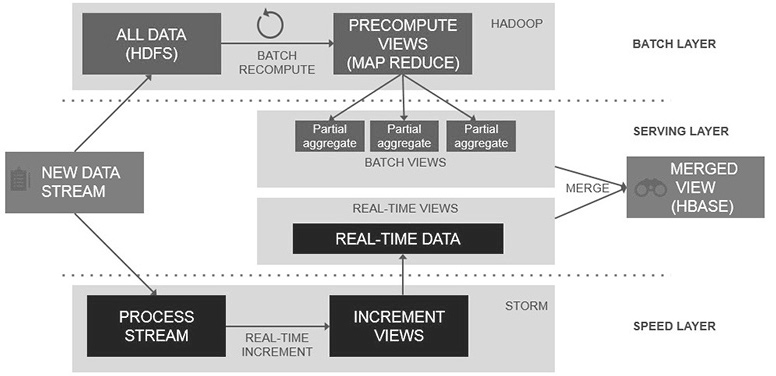
\includegraphics[width=1.0\textwidth]{images/lambda-architecture.jpg}
    \caption{Lambda Architecture}
    \label{fig:lambda-Architecture}
\end{figure}

Any query is answered through the serving layer by querying both the speed and
the batch layer. Where the badge layer periodically computes views on the
current collected data and is being outdated at the end of it's computation, the
speed layer closes this gap by constantly processing the most recent data in
near real-time fashion. \cite{marz2015big} \cite{PrpSvyOfDSPS}

\section{Centralized Event Stream}
\subsection{Need for a common data stream}
Any system which is dependent on a continuous input of data, requires a delivery
system that can provide data constantly as stream (can be
compared to an ordered message queue \todo{ref} containing events). Stream
processing systems, whether being in a lambda architecture or not, obviously
holds this requirement. On the other hand, in a big data environment there is
also the requirement of batch processing systems
(\ref{intro-datastream-batchprocessing}) being served with data. In a lambda
architecture this could be done using a stream processing framework
(\ref{intro-datastream-streamprocessing}) responsible for serving the batch
processing system with integrated data, ready for data analysis. However, an
other way of doing so would be a data store---such as the hadoop file system
(HDFS\todo{gls})---where data can be directly taken for further analysis.
The same requirement of a data store holds for any
other business intelligence system followed by the problem of the dependency of
a data store which eventually---due to the lack of an adapter---can not be
served with data by a stream processing system as comfortable as the HDFS.

\subsection{Requirements}
Facing the two types of processing events---stream- and batch
processing---together, data integration results as a common stage both systems
have to deal with. Even further, for every system an organization operates, like
the data warehouse, full-text search indexes, caches or more. The data
integration stage will be present. Additionally, stream processing systems
require a continuous incoming stream to further integrate and process where
batch processing systems on the other hand demand a given persistent set of data
to further integrate and analyze.

Further more, in terms of stream processing the requirement of low latency is
essential for any system of this type. For database systems combined with stream
processing, reliability becomes significantly important to handle critical
updates such as replicating as discussed above. In terms of batch processing
however, the demand on low latency is not as important as the availability of
well integrated data with a high throughput to be able to handle a large volume
of data in time range as low as possible.

\begin{table}[H]
\centering
\begin{tabular}{l|c|cl}
\multicolumn{1}{c|}{\textbf{}} & \textbf{Stream Processing} & \textbf{Batch
Processing} & \multicolumn{1}{c}{\textbf{}} \\ \cline{1-3}
Data Integration               & x                          & x
&                               \\
Continuous Data                & x                          &
&                               \\
Persistent Data                &                            & x
&                               \\
Low Latency                    & x                          &
&                               \\
High Throughput                     &                            & x
&
\end{tabular}
\caption{Requirements of batch and stream processing systems}
\label{table:requirements-batch-stream}
\end{table}

Note that the mentioned systems \todo{which?} do not only consume data for
integration and processing, they can also have an output. Thus, many systems are
both sources and destinations for data transfer in consequence of which a system
would then need two channels \todo{gls} per system. Obviously each output in
this constellation is intended to be consumed by 1--N system(s) again.
Connecting all of these would lead to building a custom channel between each
pair of system (see Figure \ref{fig:datapipeline_complex}). As the set of system
in an organization grows, this would clearly become a challenge to maintain.

\begin{figure}[H]
    \centering
    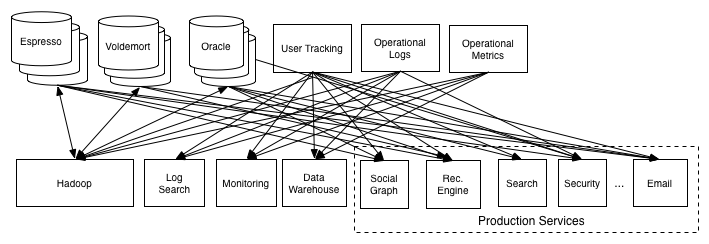
\includegraphics[width=1.0\textwidth]{images/datapipeline_complex.png}
    \caption{Complex Point-To-Point Architecture}
    \label{fig:datapipeline_complex}
\end{figure}

In this scenario several hurdles arise. The process of data integration would
have to be done for each system pair individually. At this point, an obvious
approach for a simplification would be to introduce an organization-wide
standardization of the data format. Thus, the integration process becomes 
significantly easier but still has to be done redundantly. Another problem that
remains are the tightly coupled systems. A simple change on one system could
affect one or more of it's connected systems directly, which is not only hard to
manage but also reduces the flexibility of further development of the landscape.
To extend the landscape the chances are high to touch existing systems which is
not only time intensive but also connected with risks regarding possible
failures. In fact, these are known issues of a Point-To-Point channel of
traditional messaging and are described in Section
\ref{intro-messaging-pointtopoint}.

\subsection{Central Platform as Solution}
\label{intro-datastream-centralplatform}
A more elegant and reliable approach to solve the mentioned problems would be to
introduce a central platform, that is able to support both batch and real-time
consumption and thus is able to hold the described requirements given in table
\ref{table:requirements-batch-stream}. This system can act as a single
data repository to isolated consumers and gives access to any data that is
required, as shown in figure \ref{fig:datapipeline_simple}. It aggregates
incoming events and represents an even stream for any its consumers. 

\begin{figure}[H]
    \centering
    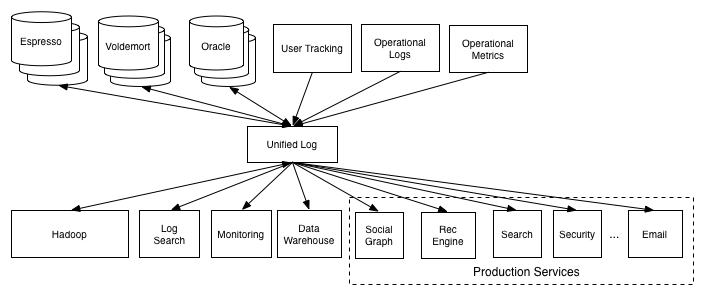
\includegraphics[width=1.0\textwidth]{images/datapipeline_simple.png}
    \caption{Broker Architecture}
    \label{fig:datapipeline_simple}
\end{figure}

In this constellation integrating a new data system---be it a data
source or a data destination---is fairly simple. Connecting it to a single
channel attached to the central platform is all what is needed to be done. Besides the
loosely coupled components, with this architecture it becomes possible to
centralize the process of data integration by doing so in a standardized way,
directly within the stream. Thus, a huge factor of complexity over the system
landscape is being reduced. In fact, this opens up a whole new set of
possibilities in organizational scalability. 

\newpage
\section{Link to Message Brokers}
As solution for a modern big data environment with huge amount of event data
which needs to be processed in different systems we need a platform which acts as
mediator to handle the incoming event as streams and provide them to several
consumers (\ref{intro-datastream-centralplatform}). This seems to be very similar to
the definition of a message broker (\ref{intro-messaging-broker}) and indeed
these two concepts can be compared. Actually an event stream can be realised
with an underlying message broker and as we already described \todo{ref}, events
can be considered as messages with the event data as payload. The central stream
platform is nothing else than a message broker which handles incoming events,
persist them in an ordered queue and provide them for the consumers which can be
stream or batch processing systems.
\begin{figure}[H]
    \centering
    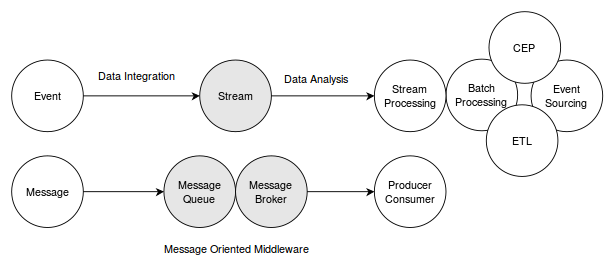
\includegraphics[width=0.8\textwidth]{images/messaging-vs-streaming.png}
    \caption{Event Stream vs Messaging}
    \label{fig:messaging-vs-streaming}
\end{figure}
The question if a message broker implementation is predestined for a big data
event stream environments is depending on its guarantees and performance. In
comparison to standard integration platform where a few applications communicate with each
other, the main challenge for a message broker in big data environment, is the
very high amount of data which needs to handled. The main demands are high
throughput and reliability in case of failures. In a survey (Chapter
\ref{survey-broker}) we examine the limits of traditional message brokers and
the needs for lately introduced systems such as Apache Kafka\cite{apachekafka},
Scribe\cite{scribe} or Flume\cite{apacheflume} and further try to compare and
categorize those systems after their strengths and weaknesses.

In the following Chapter \ref{intro-kafka} we examine capabilities of Apache
Kafka related to the functionalities of acting as a centralized event stream
platform. This gives not only a more concrete background of the components of a
state of the art message broker implementation but also serves as a basis for
the survey which is followed in Chapter \ref{survey-broker}.

%\section{Notes}

%-From traditional PCs and Smartphones to a lot of sensors who are connected to
%the interne -> Internet of Things!

%\todo[inline]{Einbringen des folgenden Statements: The nice thing about this
%architecture is that you can now have multiple consumers for the same event
%data. You can have one consumer which simply archives the raw events to some big
%storage; even if you don’t yet have the capability to process the raw events,
%you might as well store them, since storage is cheap and you can use them in
%future. Then you can have another consumer which does some aggregation (for
%example, incrementing counters), and another consumer which does something else.
%Those can all feed off the same event stream.}
